\chapter{State-of-the-Art} \label{chap:sota}

\section*{}

In this chapter we will begin by making a more in depth presentation of the
process of gene expression. This will be followed by a literature and state of
the art review in the fields of genome/\trans{} assembly and data mining.
Lastly, we will present some of the tools used in each of those areas, as well
as some relevant data representation formats for genetic data.

\section{Introduction}

- explain gene expression (DNA, genes, genome, exons, introns);\\
- explain the process of obtaining gene expression data in two steps:\\
  * genome sequencing, talk briefly about older sequencing techniques, more
  about NGS;\\
  * genome assembly, talk briefly about micro arrays, more about RNA seq and de
  novo vs guided assembly/alignment;\\

\begin{figure}[!htb]
  \begin{center}
    \leavevmode
    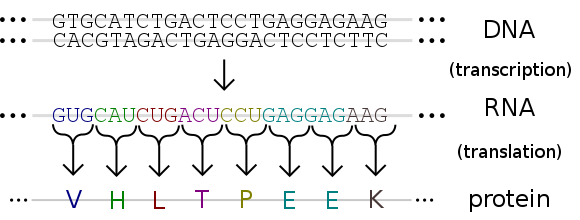
\includegraphics[width=0.6\textwidth]{gene_expr}
    \caption{Representation of the gene expression process\protect\footnotemark}
    \label{fig:arch}
  \end{center}
\end{figure}
\footnotetext{Image taken from \url{http://en.wikipedia.org/wiki/File:Genetic\_code.svg}.}

\section{Genome Assembly and \rnaseq}\label{sec:assembly}

\subsection{\rnaseq{} Tools}\label{sec:seqtools}

\subsection{Relevant Standard File Formats}\label{sec:formats}

\section{Data Mining}\label{sec:mlearning}

\subsection{Data Mining Algorithms}\label{sec:minalgo}

\subsection{Data Mining Tools}\label{sec:mintools}

\section{Chapter Conclusions}
